\documentclass{article}
\usepackage{amsmath}
\usepackage[margin=1in]{geometry}
\renewcommand{\baselinestretch}{1.5}
\usepackage{mathtools}
\usepackage{graphicx}
\usepackage{tikz}
\usetikzlibrary{arrows}
\usetikzlibrary{calc}
\author{Trixie Roque}
\title{Homework 4}
\date{05/04/15}
\begin{document}
\maketitle

	\begin{enumerate}
		\item 
			Using the Bellman-Ford algorithm, this table is created:
			\begin{center}
			\begin{tabular} {| c || c | c | c | c | c | c |}
				
				\hline
				Nodes $\backslash$ Iterations	&	0	&	 1	 &	 2	 &	 3	 &	 4	&	 5 \\ \hline \hline
				S 	   	&	0	&	 0	 &	 0	 &	 0	 &	 0	&	 0 \\ \hline
				A 	   	& $\infty$  &	7	 &	 7	 &	 7	 & 	 7	& 	 7 \\ \hline
				B 	   	& $\infty$	&  $\infty$  & 	11	 & 	11 	 & 	11	& 	11 \\ \hline
				C 	   	& $\infty$	&  	6  	 & 	5   	 & 	 5   	 & 	 5   	& 	5 \\ \hline
				D 	   	& $\infty$	&  $\infty$  &  	8  	 &  	 7 	 &	 7  	&	 7\\ \hline
				E 	   	& $\infty$	&  	6	 &  	6  	 & 	 6 	 &  	 6	& 	6 \\ \hline
				F         	& $\infty$	&  	5  	 &  	4 	 &  	 4	 & 	 4 	&	 4 \\ \hline
				G 	   	& $\infty$	&  $\infty$  &  $\infty$ & 	 9  	 &  	 8  	&	 8 \\ \hline
				H 	   	& $\infty$	&  $\infty$  &  	9  	 & 	 7  	 &  	 7  	& 	7 \\ \hline
				I 	   	& $\infty$	&  $\infty$  &  $\infty$ &  $\infty$ &  	 8 	& 	7 \\ \hline
			\end{tabular}
			\end{center}
	
		\item
			The method proposed by Professor F. Lake is incorrect. A possible counterexample to this method is if the shortest path of the original graph has negative edge weights:
			\begin{center}
			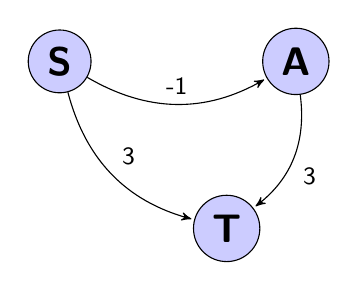
\begin{tikzpicture}[->,>=stealth',shorten >=1pt,auto,node distance=3cm,thin,main node/.style={circle,fill=blue!20,draw,font=\sffamily\Large\bfseries}]
			
        				\node[main node] (S) {S};
        				\node[main node] (A) [right of=S]{A};
        				\node[main node] (T) [below right of=S]{T};
				
				\path[every node/.style={font=\sffamily\small}]
				(S) edge [bend right] node {-1} (A) 
				(A) edge [bend left] node {3} (T)
				(S) edge [bend right] node {3} (T);
				
			\end{tikzpicture}
			\\
			Original Graph
			\end{center}
			
			This graph's shortest path from $S$ to $T$ costs 2: $S \Longrightarrow A \Longrightarrow T$
			\\
			Using Professor F. Lake's method, the edge weights will all be positive and the shortest path will be different: \\
			
			\begin{center}
			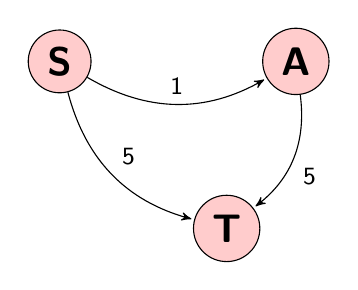
\begin{tikzpicture}[->,>=stealth',shorten >=1pt,auto,node distance=3cm,thin,main node/.style={circle,fill=red!20,draw,font=\sffamily\Large\bfseries}]
			
        				\node[main node] (S) {S};
        				\node[main node] (A) [right of=S]{A};
        				\node[main node] (T) [below right of=S]{T};
				
				\path[every node/.style={font=\sffamily\small}]
				(S) edge [bend right] node {1} (A) 
				(A) edge [bend left] node {5} (T)
				(S) edge [bend right] node {5} (T);
				
			\end{tikzpicture} \\
			Modified graph
			\end{center}
			Here, the shortest path costs 5: $S \Longrightarrow T$\\
			
			\item
			Proof: \\
			Since we only need to prove $O$, we have to find an upper bound so that $O(W|V| + E)$. Given a graph whose edge weights are integers in the range $0, 1, . . . , W$ , where $W$ is a relatively small number, the maximum weight that any of the edge can have is $W$. Also, given $V$ number of vertices, updating a vertex using Dijkstra's algorithm will only take at most $|V| - 1$ times since the vertex itself will not be looping to itself. Then, using Dial's implementationusing of using doubly-linked lists which have the properties that allow constant time checking whether a graph is empty/nonempty, and deleting/adding a node, the edges will only be $O(E)$. Thus, we can have $O(W|V| + E)$ complexity. \\
			(Source: http://www.ece.northwestern.edu/~dda902/336/hw5-sol.pdf)
			\\
			
			\item
			(a) Prim's algorithm produced the table below
			\begin{center}
			\begin{tabular} {| c || c | c | c | c | c | c | c | c |}
			\hline
			Set S 				& 	A & 	B    & 	C	 & 	D 	    & E 	& F 		& G 		& H \\ \hline \hline
			$A$ 					& 0/nil & 1/A   & $\infty$/nil & $\infty$/nil & 4/A 	& 8/A 	& $\infty$/nil &$\infty$/nil \\ \hline
			$A, B$ 				&    	   &  	      & 2/B 		& $\infty$/nil & 4/A 	& 6/B 	& 6/B 	& $\infty$/nil \\ \hline
			$A, B, C$ 				&	   &         &  		& 3/C	 &  4/A 	& 6/B	& 2/C 	& $\infty$/nil \\ \hline
			$A, B, C, G$ 			&    	   &         &  		&  1/G	& 4/A 	& 1/G 	&	 	& 1/G \\ \hline
			$A, B, C, G, D$ 		&    	   &         &  		&  		&  4/A 	& 1/G 	&	 	& 1/G \\ \hline
			$A, B, C, G, D, F$ 		&    	   &         & 		&  		&  4/A	&		&	 	& 1/G \\ \hline
			$A, B, C, G, D, F, H$ 	&    	   &         &  		&  		&  4/A 	&	 	&  		&  \\ \hline
			\end{tabular}
			\end{center}
			(b) We start with disjoint nodes
			\begin{center}
			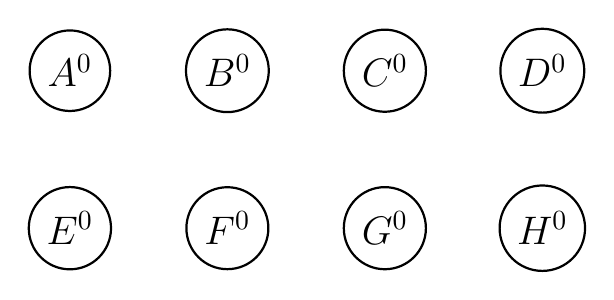
\begin{tikzpicture}[->,>=stealth',shorten >=1pt,auto,node distance=2cm,thick,main node/.style={circle,draw,font=\sffamily\Large\bfseries}]
				
				\node[main node] (A) {$A^0$};
  				\node[main node] (B) [right of = A] {$B^0$};
				\node[main node] (C) [right of=B] {$C^0$};
  				\node[main node] (D) [right of = C] {$D^0$};
				\node[main node] (E) [below of =A] {$E^0$};
				\node[main node] (F) [below of = B] {$F^0$};
				\node[main node] (G) [below of = C] {$G^0$};
				\node[main node] (H) [below of = D] {$H^0$};

    				\end{tikzpicture}
			\end{center}
			Then using Kruskal's algorithm, we take the edges with the smallest weight. In this case, we start with length = 1: (A, B), (G, D), (G, F), (G, H) so we have: \\
			$A^0 \Longrightarrow B^1$, $G^0 \Longrightarrow D^1$, $G^0 \Longrightarrow F^1$, $G^0 \Longrightarrow H^1$ \\
			Then we have the sets \{A, B\}, \{D, G\} \{F, G\}, \{H, G\}, but since three of these sets are not disjoint, we actually have the disjoint sets \{A, B\} and \{D, F, G, H\} in order to cover the edges with length 1. \\
			\begin{center}
			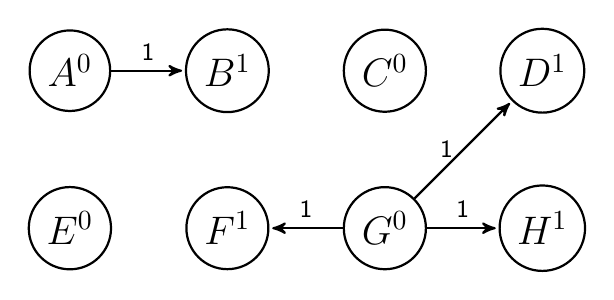
\begin{tikzpicture}[->,>=stealth',shorten >=1pt,auto,node distance=2cm,thick,main node/.style={circle,draw,font=\sffamily\Large\bfseries}]
				
				\node[main node] (A) {$A^0$};
  				\node[main node] (B) [right of = A] {$B^1$};
				\node[main node] (C) [right of=B] {$C^0$};
  				\node[main node] (D) [right of = C] {$D^1$};
				\node[main node] (E) [below of =A] {$E^0$};
				\node[main node] (F) [below of = B] {$F^1$};
				\node[main node] (G) [below of = C] {$G^0$};
				\node[main node] (H) [below of = D] {$H^1$};
				
    				\path[every node/.style={font=\sffamily\small}]
    				(A) edge node [above] {1} (B)
				(G) edge node [above] {1} (F)
				(G) edge node [left] {1} (D)
				(G) edge node [above] {1} (H);

    				\end{tikzpicture}
			\end{center}
			
			Then, length = 2 edges are (B, C), (C, G) so we have: \\
			$A^0 \Longrightarrow B^1 \Longrightarrow C^1$, $C^0 \Longrightarrow G^1$ \\
			Since these aren't disjoint sets, we actually have the set \{A, B, C, D, G, F, H\} such that 
			
			\begin{center}
			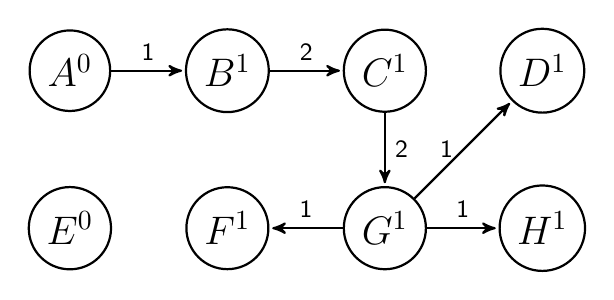
\begin{tikzpicture}[->,>=stealth',shorten >=1pt,auto,node distance=2cm,thick,main node/.style={circle,draw,font=\sffamily\Large\bfseries}]
				
				\node[main node] (A) {$A^0$};
  				\node[main node] (B) [right of = A] {$B^1$};
				\node[main node] (C) [right of=B] {$C^1$};
  				\node[main node] (D) [right of = C] {$D^1$};
				\node[main node] (E) [below of =A] {$E^0$};
				\node[main node] (F) [below of = B] {$F^1$};
				\node[main node] (G) [below of = C] {$G^1$};
				\node[main node] (H) [below of = D] {$H^1$};
				
    				\path[every node/.style={font=\sffamily\small}]
    				(A) edge node [above] {1} (B)
				(B) edge node [above] {2} (C)
				(C) edge node [right] {2} (G)
				(G) edge node [above] {1} (F)
				(G) edge node [left] {1} (D)
				(G) edge node [above] {1} (H);

    				\end{tikzpicture}
			\end{center}
			Then finally adding node E, since we can only use edges (A, E) with length = 4 and (F, E) with length = 5, we choose the edge with the smallest weight, (A, E), just like how we have been doing the other edges. Then we have the set \{A, B, C, D, E, G, F, H\} 
			
			\begin{center}
			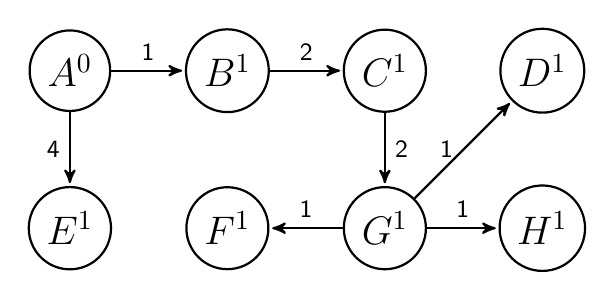
\begin{tikzpicture}[->,>=stealth',shorten >=1pt,auto,node distance=2cm,thick,main node/.style={circle,draw,font=\sffamily\Large\bfseries}]
				
				\node[main node] (A) {$A^0$};
  				\node[main node] (B) [right of = A] {$B^1$};
				\node[main node] (C) [right of=B] {$C^1$};
  				\node[main node] (D) [right of = C] {$D^1$};
				\node[main node] (E) [below of =A] {$E^1$};
				\node[main node] (F) [below of = B] {$F^1$};
				\node[main node] (G) [below of = C] {$G^1$};
				\node[main node] (H) [below of = D] {$H^1$};
				
    				\path[every node/.style={font=\sffamily\small}]
    				(A) edge node [above] {1} (B)
				(A) edge node [left] {4} (E)
				(B) edge node [above] {2} (C)
				(C) edge node [right] {2} (G)
				(G) edge node [above] {1} (F)
				(G) edge node [left] {1} (D)
				(G) edge node [above] {1} (H);

    				\end{tikzpicture}
			\end{center}
			
		\item 
			See SubsetSum.java in GitHub repo trixr4kdz/cmsi282/homework4.
			
		\item
			See BoardingSchool.java in GitHub repo trixr4kdz/cmsi282/homework4.
			
	\end{enumerate}
	
\end{document}